% Created 2025-01-02 Thu 18:23
% Intended LaTeX compiler: pdflatex
\documentclass[11pt]{article}
\input{../../../preamble.tex}
% setting up title page
\title{
  
\includegraphics[width=0.4\textwidth]{fmf_logo}\\
  {\small Oddelek za fiziko} \\
  {Elektronsko spinska resonanca}\\
  {\small Poročilo pri FP5}\\
}
\date{}
\author{ Kristofer Č. Povšič, 28211104 \\[5 cm]
 \small  Asistent: Tilen Knaflič \\
}
\begin{document}

\maketitle
\tableofcontents

\section{Uvod}\label{sec:org2f7b62e}
Za spektroskopijo z elektronsko spinsko resonanco se pogosto uporablja sinonim elektronske magnetne resonance. Magnetna resonančna spektroskopija se imenuje, ker merimo prehod med energijskimi nivoji prostih elektronov v magnetnem polju. Princip delovanja je podoben kot pri jedrski magnetni resonanci, le da so frekvence mnogo višje. Pri nižjih frekvencah in odgovarjajočem magnetnem polju vseeno pride do zanimivih pojavov.

Elektron je delec s spinom \(S = \frac{1}{2}\) in ima po klasični teoriji magnetni moment, katerega velikost je \emph{Bohrov magneton} \(\mu_B = e \hbar/ 2 m_e = 9.27 10^{-24} \mathrm{J} / \mathrm{T}\). V zunanjem magnetnem polju imamo dve možnosti projekcije vrtilne količine. Vzporedno z magnetnim poljem \(B_0\), kjer je magnetno kvantno število \(m_s = \frac{1}{2}\) in nasprotno s poljem \(m_s = - \frac{1}{2}\). Med tema stanjema je energijska razlika \(\Delta E\):

\[ \Delta E = E_{\text{up}} - E_{\text{down}} = g \mu_B B_0
\]

kjer je \(g\) Landejev faktor in je za prost elektron (z upoštevkom relativističnih popravkov) enak \(2.0023192\). Landejev faktor je odvisen tudi od kemične vezave in elektronskega okolja. Prehode med tema dvema nivojema lahko vzbujamo z elektromagnetnih sevanjem, ki je dovolj energetično, ai. izpolnjuje pogoje

\[ \Delta E = g \mu_B B_0 = h \nu
\]

Tako smo dobili zvezo med frekvenco in resonančno vrednostjo magnetnega polja. Energijska razlika \(\Delta E\) je relativno majhna v primerjavi z vidno ali IR spektroskopijo, zato so signali precej šibki. Relativno populacijo obeh energijskih nivojev podaja Boltzmannova porazdelitev

\[ \frac{n_2}{n_1} = e ^{- \frac{\Delta E}{k_B T}} = e ^{- \frac{h \nu}{k_B T}}
\]

kjer je \(k_B\) Boltzmannova konstanta in \(T\) absolutna temperatura. Zaradi interakcij elektrona s kristalno mrežo, z drugimi elektroni ali jedri, resonančne črte niso ostre, ampak razširjene ali razcepljene.
\subsection{Eksperiment}\label{sec:org7199d4b}

V našem primeru imamo vzorec \textbf{DPPH} (2, 2-diphenil-1-pikrilhidrazil), ki se nahaja v tuljavi resonančnega regenerativnega oscilatorja. Ko zunanje magnetno polje \(B_0\) doseže vrednosti, ki izpolnjuje resonančni pogoj, nastopi absorpcija visoko frekvenčnega valovanja in amplituda oscilacij oscilatorja pade. Oscilacije preko diode opazujem na osciloskopu.

Dodatno si olajšamo z modulacijo magnetnega polja. Amplituda modulacije je običajno manjša od širine črte, kar pomeni, da dobimo signal modulacijske, katerega amplituda je proporcianalna odvodu absorcpijske črte v odvisnosti od statične komponente polja.

Signal na osciloskopu je šibek in ne izstopa od šuma, zato uporabimo fazni detektor. Ta ima na voljo referenčni signal \(U_{ref} = U_0 \cos (\omega t + \phi)\), kar je v našem primeru napetosti, ki napaja modulacijske tuljave. Signal \(U_{sig} = A(t) \cos (\omega t)\) je usmerjen izhod regenerativnega oscilatorja delno prekrit s šumom in iste frekvence \(\omega\). Med njima je fazna razlika \(\phi\).

Fazni detektor napravi produkt obeh singalov kot analogni množilec

\[ U_{out} = U_{ref} U_{sig} = \frac{1}{2} A(t) \left[ \cos \phi + \cos (2\omega + \phi) \right]
\]
S tem smo dosegli, da je nosilna frekvenca signala \(A(t)\) enaka nič. Drugega člea pa se preprosto znebimo z RC filtrom.

\section{Potrebščine}\label{sec:org6464457}
\begin{itemize}
\item vzorec
\item refenerrativni oscilator
\item osciloskop
\item modulacijske tuljave in njihov napajalec
\item fazni detektor
\end{itemize}

\section{Naloge}\label{sec:org74240be}
\begin{itemize}
\item z vzorcem DPPH kot merjencem določi \(g\) faktor prostega elektrona in razmerje \(B/ \nu\).
\item izmeri širino absorcpijske črte
\end{itemize}

\section{Meritve in izračuni}\label{sec:org1f22431}

Diagonalo tuljave sem izračunal po formuli

\[ d = \sqrt{l ^2 + (r_1 ^2 + r_2 ^2)}
\]

in dobil za izmerjene \(r_1 = (4.5 \pm 0.1) \mathrm{cm}\), \(r_2 = (8.7 \pm 0.1) \mathrm{cm}\) in dolžina tuljave \(l = (13.2 \pm 0.1)\)

\[ d = (18.6 \pm 0.1) \mathrm{cm}
\]

Prav tako \(g\) faktor izrazimo kot

\[ g = \frac{h \nu}{\mu_B B_0}
\]

Magnetno poljsko gostoto izrazimo z

\begin{equation}
\label{eq:1}
B_0 = \frac{N \mu_0 I}{d}
\end{equation}

Izmeril in naredil sem grafe odvoda absorpcijske črte pri \(80, 85, 90 \ \mathrm{MHz}\).

\begin{slika}[H]
  \centering
  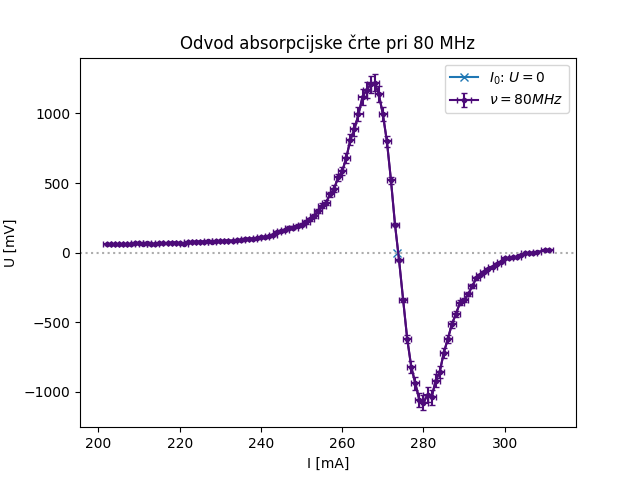
\includegraphics[width=.9\linewidth]{figures/abs_crte.png}
  \caption{\small Graf prikazuje odvod absorcpijske črte za 3 frekvence: $80, 85, 90 \ \mathrm{MHz}$.}
\end{slika}

Za \(B_0\) sem vzel vrednost toka, ki je označena z \(\times\) na grafu in je točka, kjer naj bi bila napetost med maksimumom in minimumom enaka 0. Preko enačbe \ref{eq:1} sem dobil vrednosti

\begin{align*}
  B_{080} &= (2.86 \pm 0.02) \mathrm{mT} \\
B_{085} &= (3.04 \pm 0.02) \mathrm{mT} \\
B_{090} &= (3.23 \pm 0.02) \mathrm{mT}
\end{align*}

Za razdalja med ekstremoma sem odčital in izračunal preko enačbe \ref{eq:1} sem dobil

\begin{align*}
\Delta B_{80} &=  (0.12 \pm 0.01) \mathrm{mT} \\
\Delta B_{85} &= (0.13 \pm 0.02) \mathrm{mT} \\
\Delta B_{90} &= (0.14 \pm 0.01) \mathrm{mT}
\end{align*}

Razmerje \(\nu / B_0\) pa je enako

\begin{align*}
  \left(\frac{\nu}{B_0}\right)_{80} &= (27.8 \pm 0.2) \frac{\mathrm{GHz}}{\mathrm{T}} \\
  \left(\frac{\nu}{B_0}\right)_{85} &= (27.9 \pm 0.2) \frac{\mathrm{GHz}}{\mathrm{T}}\\
  \left(\frac{\nu}{B_0}\right)_{90} &= (27.8 \pm 0.2) \frac{\mathrm{GHz}}{\mathrm{T}}
\end{align*}

\begin{slika}[H]
  \centering
  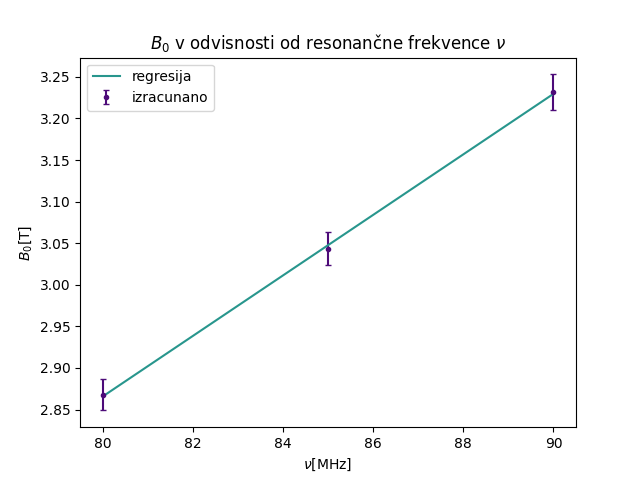
\includegraphics[width=.9\linewidth]{figures/gfaktor.png}
  \caption{\small Graf prikazuje regresijo premice, katere vrednost nam poda faktor $g$.}\label{fig:gfaktor}
\end{slika}

Za \(g\) vrednost sem regresiral premico na dane podatke in iz grafa \ref{fig:gfaktor} dobil vrednost

\[ g = 1.96 \pm 0.04
\]

\section{Komentar}\label{sec:org17b2783}

Izračunani podatki se zdijo smiselni. Meritev je tudi potekala brez kakršnihkolih večjih težav.
\end{document}
